\section{Regressão Linear}

Procedimentos Univariados

Teste K-S e Shapiro-Wilk

Análise de Outlier - Boxplot

Verificar os slides ``Introdução ao SPSS"

	\subsection{Método da Linha Reta}
	
		``É o tipo mais simples de ajustamento de curvas, cuja equação é
		
		\bigskip		
		
		{\Large $ Y = a + bX $} \ ,
		
		\bigskip
		
		onde  $ X $ e $ Y $ são variáveis e $ a $ e $ b $ são as constantes.

		Assim, dados dois pontos quaisquer $ (X1,Y1) $ e $ (X2,Y2) $ dessa reta, as constantes $ a $ e $ b $ podem ser determinadas" \cite{torres} .
	
		\subsubsection{Equação da Reta}
		
			``Podemos também considerar a forma mais comum de representar a função de 1º grau (função linear), ou seja, 
			
			\bigskip
			
			{\Large $ y = mx + n $} \ ;
			
			\bigskip
			
			onde $ b = m $ é coeficiente angular e $a = n$ é o coeficiente linear" . \cite{morettin}
			
			\bigskip			
			
			{\Large $ m = \cfrac{\Delta y}{\Delta x} = \cfrac{y_2 - y_1}{x_2 - x_1}$}
			
	\subsection{Método dos Mínimos Quadrados}

		``A reta dos mínimos quadrados que se ajusta ao conjunto de pontos, tem a equação:

		\bigskip

		{\Large $ Y = a + bX + e $} \ ,

		\bigskip

		sendo $ a + bX $ a equação da reta, e $ e $ o termo erro. Este último termo tem de ser incluído porque o valor de Y não será dado exatamente pelo ponto da reta a ser encontrada" \cite{torres}.

		\bigskip

		``Podemos dizer então, que o erro dá conta de todos os eventos que são difíceis de medir, mas que são (supostamente) aleatórios. Mais do que isso, se o modelo (no nosso caso uma reta) estiver corretamente especificado, podemos supor que o erro, em média, será zero. Isto é, a probabilidade do erro ser $ x $ unidades acima da reta é a mesma de ser $ x $ unidades abaixo.

		Essa é a primeira hipótese: $ E(e_i) = 0 $ \ " \cite{torres}.

		\bigskip			
		
		``O próximo passo é estimar a reta de regressão:
		
		\bigskip
		
		{\Large $ a = \cfrac{\sum y - b \sum x}{n} $}
		
		\bigskip
		
		{\Large $ b = \cfrac{n \sum xy - \sum x \sum y}{n \sum x^{2} - (\sum x)^{2}} $}
		
		\bigskip
		
		$ a = $ o valor de $ y_{i} $ \ , quando o $ x_{i} = 0 $ \ ou o intercepto da reta no eixo $ y $ \ .
		
		$ b = $ o valor do coeficiente angular, que indica a inclinação da reta" \cite{torres}.

	\subsection{Coeficiente de Correlação Amostral de Pearson ($ r $)}
		
		``O coeficiente de correlação amostral de Pearson é indicado por $ r $ e calculado através da fórmula:
		
		\bigskip
		
		{\Large $ r = \cfrac{n \sum X Y - ( \sum X) ( \sum Y)}{ \sqrt{ [ n ( \sum X^{2} ) - ( \sum X)^{2}] [n ( \sum Y^{2}) - ( \sum Y)^{2} ] }} $}
		
		\bigskip
		
		onde,
		
		\bigskip
		
		$ r = 1 \Rightarrow $ Correlação perfeita positiva;
		
		$ r = 0 \Rightarrow $ Correlação nula;
		
		$ r = -1 \Rightarrow $ Correlação perfeita negativa". \cite{torres}
		
		\bigskip
		
		O coeficiente de correlação \textbf{populacional} de Pearson é indicado por \textbf{$ \rho $}.
		
		\paragraph{Premissas \cite{torres}}
		
			\begin{enumerate}[label=(\alph*)]
		
				\item as duas variáveis envolvidas são \textbf{aleatórias e contínua}s;
				
				\item as duas variáveis \textbf{apresentam uma distribuição normal}.			
			
			\end{enumerate}
			
	\subsection{Coeficiente de Determinação ($ r^{2} $ ou $ R^{2} $)}
			
		``O coeficiente de determinação \textbf{$ r^{2} $} (amostral) ou \textbf{$ R^{2} $} (populacional) mede o grau de ajustamento da reta de regressão aos dados observados.

		\bigskip
		
		O coeficiente de determinação representa a relação entre a variação explicada pelo modelo e a variação total, ou em outras palavras, indica a proporção da variação total da variável dependente $ y $ que é explicada pela variação da variável independente $ x $ \ ". \cite{torres}
			
	\subsection{Erro Padrão da Estimativa Amostral ($ s_{e} $)}
			
		``O erro padrão da estimativa [amostral] calcula a dispersão dos resíduos (diferença entre valores reais e preditos) dos valores amostrados ao redor da reta de regressão. Quanto maior a dispersão, menor a precisão das estimativas". \cite{torres}
			
		``Pode ser calculado pela fórmula que segue:
		
		\bigskip
		
		{\Large $ s_{e} = \sqrt{\cfrac{\sum y^{2} - a \sum y - b \sum xy}{n - 2}} $}
		
		\bigskip
		
		onde,
		
		$ s_{e} = $ o erro padrão associado a $ y $ \ ;
		
		$ n = $ número de observações". \cite{torres}

	\subsection{Erro Padrão do Coeficiente Angular Amostral ($ s_{b} $)}

		``O cálculo do erro padrão do coeficiente angular amostral $ b $ é importante para poder construir o intervalo de confiança e efetuar os testes de hipóteses apropriados para o coeficiente angular $ \beta $ \ ". \cite{torres}

		``Algebricamente, o erro padrão de $ b $ (coeficiente angular) pode ser apresentado por meio da seguinte equação:
		
		\bigskip
		
		{\Large $ s_{b} = \cfrac{s_{e}}{\sqrt{(n-1) \cdot S_{x}^{2}}} $}
		
		\bigskip
		
		onde,
		
		$ s_{e} = $ o erro padrão associado a $ y $ \ ;

		$ n = $ número de observações;
		
		$ S_{x}^{2} = $ variância de $ x $ (variável independente)". \cite{torres}

		\bigskip

		Vale relembrar a forma de calcular $ S_{x}^{2} $ e $ \bar X $.
		
		\bigskip
		
		{\Large $ S^{2} = \cfrac{\sum (X_{i} - \bar X)^{2}}{n-1} $}
		
		\bigskip
		
		{\Large $ \bar X_{x} = \cfrac{\sum X_{i}}{n} $}

	\subsection{Erro Padrão do Coeficiente Linear Amostral ( $ s_{a} $ )}

		``Algebricamente, o erro padrão [amostral] de $ a $ (coeficiente linear) pode ser apresentado por meio da seguinte equação:
		
		\bigskip
		
		{\Large $ s_{a} = s_{e} \cdot \sqrt{\cfrac{1}{n} + \cfrac{\bar X^{2}}{(n - 1) \cdot S_{x}^{2}}} $}
		
		\bigskip
		
		onde,
		
		$ s_{e} = $ o erro padrão associado a $ y $ \ ;

		$ n = $ número de observações;
		
		$ \bar X = $ média de $ x $ (variável independente);
		
		$ S_{x}^{2} = $ variância de $ x $ (variável independente)". \cite{torres}

	\subsection{Erro Padrão do Coeficiente de Correlação Populacional ($ s_{\rho} $)}
	
		``O erro padrão do coeficiente de correlação populacional, geralmente expresso pela letra rô ( $ \rho $ ), pode ser calculado pela seguinte expressão:
	
		\bigskip
		
		{\Large $ s_{\rho} = \sqrt{\cfrac{1 - r^{2}}{n - 2}} $}
		
		\bigskip
		
		onde,
		
		$ r^{2} = $ o erro padrão associado a $ y $ \ ;

		$ n = $ número de \textbf{pares analisados}". \cite{torres}
	
	\subsection{Utilizando a Distribuição t (\textit{Student}) para Testar a Nulidade dos Estimadores \cite{torres}}
	
		\subsubsection{Premissas}
			
			\begin{enumerate}[label=(\alph*)]
		
				\item as duas variáveis envolvidas são \textbf{aleatórias e contínua}s;
				
				\item as duas variáveis \textbf{apresentam uma distribuição normal}.
			
			\end{enumerate}
			
		\subsubsection{Coeficiente Angular ($ \beta $)}

			{\Large $ t = \cfrac{b - \beta_{0}}{s_{b}} $}

			\paragraph{Intervalo de Confiança}

				{\Large $ b \pm t \cdot s_{b} $}

			\paragraph{Teste de Hipóteses}

				$
					\begin{cases}
			        \mathsf{H}_{0} : & \beta = 0 \\
			        \mathsf{H}_{a} : & \beta \neq 0
			        \end{cases}
				$

		\subsubsection{Coeficiente Linear ($ \alpha $)}

			{\Large $ t = \cfrac{b - \alpha_{0}}{s_{a}} $}

			\paragraph{Intervalo de Confiança}
				
				{\Large $ a \pm t \cdot s_{a} $}
				
			\paragraph{Teste de Hipóteses}

				$
					\begin{cases}
			        \mathsf{H}_{0} : & \alpha = 0 \\
			        \mathsf{H}_{a} : & \alpha \neq 0
			        \end{cases}
				$

		\subsubsection{Coeficiente de Correlação ($ \rho $)}

			{\Large $ t = \cfrac{b - \rho_{0}}{s_{\rho}} $}

			\paragraph{Intervalo de Confiança}

				{\Large $ r \pm t \cdot s_{\rho} $}

			\paragraph{Teste de Hipóteses}

				$
					\begin{cases}
			        \mathsf{H}_{0} : & \rho = 0 \\
			        \mathsf{H}_{a} : & \rho \neq 0
			        \end{cases}
				$

		\subsubsection{Projeção ($ \hat Y_{i} $)}

			\paragraph{Intervalo de Confiança}

				{\Large $ \hat y_{i} \pm t \cdot s_{e} \cdot \sqrt{\cfrac{1}{n} + \cfrac{(x_{i} - \bar X)^{2}}{\sum \limits^{n}_{i=1} x^{2}_{i} - \cfrac{\left( \sum \limits^{n}_{i=1} x_{i} \right) ^{2}}{n}}} $}
				
	\subsection{Hipóteses do teste K-S e Shapiro-Wilk \cite{torres}}
		
		Ambos são testes de aderência à distribuição normal. Para os testes de Kolmogorov-Smirnov (\textbf{K-S}) e \textbf{Shapiro-Wilks} as hipóteses normalmente utilizadas são as abaixo. \cite{torres}

		\bigskip

		$
			\begin{cases}
			\mathsf{H}_{0} : & \text{os dados apresentam distribuição normal} \\
			\mathsf{H}_{a} : & \text{os dados não apresentam distribuição normal}
			\end{cases}
		$	
	
		\bigskip	
	
		Logo, para esses testes, quando o sigma estiver acima de $ 5 \% $ (caso seja esse o nível de significância utilizado) deve se considerar que os dados apresentação distribuição normal.
		
		\bigskip
		
		O teste de Kolmogorov-Smirnov \textbf{K-S} é utilizado para amostras grandes, quando \textbf{$ n > 50 $} . Para amostras pequenas utilize o teste de \textbf{Shapiro-Wilks}. \cite{torres}
	
	\subsection{Avaliação do Modelo Utilizando o SPSS}

		\textbf{Pressupostos da Regressão}

			\begin{enumerate}[label=(\alph*)]
		
				\item Qualidade do Ajustamento;
				\item Teste t;
				\item Teste F;
				\item Normalidade dos Resíduos;
				\item Homocedasticidade dos Resíduos (Variância Constante);
				\item Linearidade;
				\item Ausência de Autocorrelação dos Resíduos;
				\item Ausência de Multicolinearidade entre as Variáveis Independentes. \cite{torres}		
			
			\end{enumerate}

		\subsubsection{Qualidade do Ajustamento}

			Verifique o valor do \textbf{$ R^{2} $ ajustado} ou \emph{Adjusted $ R^{2} $}.
			
			Quanto maior o ajustamento mais o modelo explica o que está se estudando. \cite{torres}

			\begin{figure}[H]
				\centering
				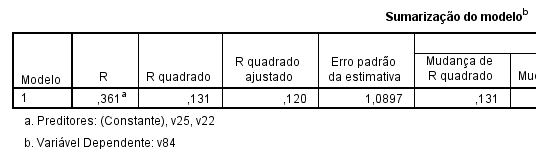
\includegraphics[height=4cm]{images/rl_ajustamento}
			\end{figure}

		\subsubsection{Teste t}

			Verifique a nulidade das variáveis.
			
			Caso exista, uma opção é retirar as variáveis nulas e rodar o modelo de novo. Outra opção é rodar uma regressão fatorial.

			É possível manter a variável mesmo nula caso ela seja muito importante para o modelo. \cite{torres}

			\begin{figure}[H]
				\centering
				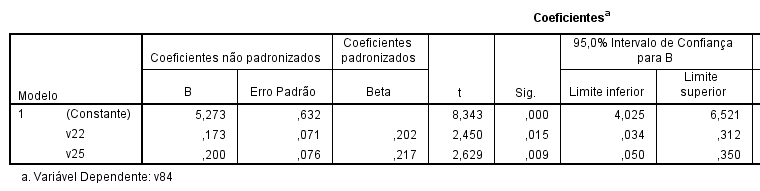
\includegraphics[height=4cm]{images/rl_teste-t}
			\end{figure}

		\subsubsection{Teste F}

			Ao verificar os resultados da ANOVA (\emph{Analysis of Variance}), veja se o sigma de F está abaixo de $ 5\% $ (caso seja esse o nível de significância desejado).

			\begin{figure}[H]
				\centering
				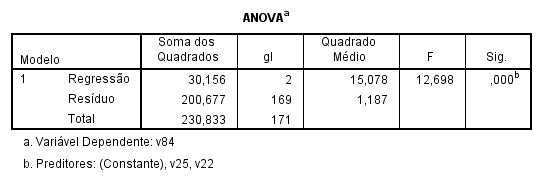
\includegraphics[height=4cm]{images/rl_anova}
			\end{figure}

			As premissas dos testes de hipóteses de F são as mesma do teste t. Seguem elas abaixo.

			\bigskip

			$
				\begin{cases}
					\mathsf{H}_{0} : & R^{2} = 0 \\
					\mathsf{H}_{a} : & R^{2} \neq 0
				\end{cases}
			$	

		\subsubsection{Normalidade dos Resíduos}

			É importante olhar a normalidade dos resíduos para verificar se eles estão ajustados ao modelo (neste caso linear) e também para verificar a presença/ausência de outliers.
			
			No SPSS isso se faz explorando a explorando os \textbf{resíduos standardizados Z} ou \emph{Standardized Residual Z - ZRE}. \cite{torres}

			\begin{figure}[H]
				\centering
				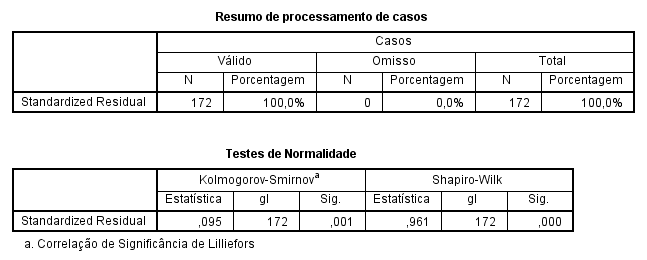
\includegraphics[height=6cm]{images/rl_normalidade-de-residuos}
			\end{figure}

		\subsubsection{Homocedasticidade dos Resíduos (Variância Constante)}

			``A presença de variâncias não homogêneas é uma violação de um dos pressupostos da regressão, conhecida como heterocedasticidade.
			
			\bigskip
			
			\textbf{Possíveis causas}: outliers; erro de especificação das variáveis; \textbf{erro na função matemática} (Ela pode ser não-linear. No marketing as disciplinas não passam por regressão não-linear, logo, nos exercícios a opção nunca será essa. O correto é testar outros modelos antes de retirar os outliers.), entre outros.
			
			\bigskip
			
			\textbf{Soluções possíveis}: transformar variáveis ou estimação da regressão via mínimos quadrados ponderados; retirada de outliers". \cite{torres}

			\bigskip

			Para analisar a homocedasticidade no SPSS, \textbf{gere um gráfico de dispersão simples} com a variável \emph{Studentized Residual - SRE} no eixo $ x $ e a variável \emph{Standardized Predicted Value - ZPR} no eixo $ y $ .

			\begin{figure}[H]
				\centering
				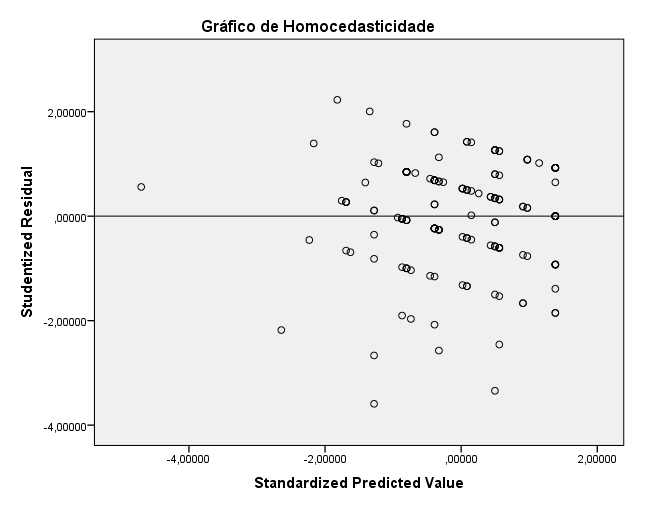
\includegraphics[height=6cm]{images/rl_homocedasticidade}
			\end{figure}

		\subsubsection{Linearidade}

			O diagnóstico de linearidade pode ser feito pelo diagrama de dispersão [o mesmo realizado para a avaliação de homocedasticidade, que dá uma boa ideia sobre sua linearidade em torno das observações das variáveis dependentes e independentes.

			\bigskip
			
			Suas possíveis causas e soluções são as mesmas apresentadas para Variância Constante (pressuposto anterior).

		\subsubsection{Ausência de Autocorrelação dos Resíduos}

			``A análise da autocorrelação dos resíduos pode ser feita através do Teste de Durbin-Watson, cujas hipóteses são:
			
			\bigskip

				$
					\begin{cases}
					\mathsf{H}_{0} : & \text{não existe autocorrelação dos resíduos} \\
					\mathsf{H}_{a} : & \text{existe autocorrelação dos resíduos}
					\end{cases}
				$

			\bigskip

			Quero que não exista autocorrelação, pois a violação leva a erro na estimação dos parâmetros.
			
			\bigskip
			
			A idéia da chamada autocorrelação serial é que os resíduos
contém mais informação sobre a variável dependente do que aquilo que foi “filtrado” pelas variáveis explicativas. Em termos técnicos, o resíduo ainda pode ser sistematizado.

			\bigskip

			Exemplos de autocorrelação são normalmente encontrados em trabalhos que utilizam séries de tempo como dados de análise.
			
			\bigskip
			
			A autocorrelação dos resíduos depende do valor do teste de Durbin-Watson, cuja interpretação é:
			
			\bigskip
			
			\textbf{Valores próximos de 2, não existe autocorrelação dos resíduos;}
			
			\bigskip
			
			Valores próximos de Zero, significa autocorrelação positiva;
			
			Valores próximos de 4, significa autocorrelação negativa". \cite{torres}

			\begin{figure}[H]
				\centering
				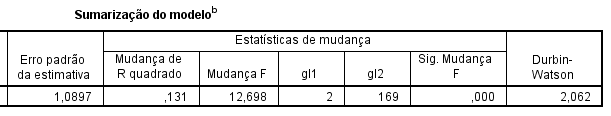
\includegraphics[height=3cm]{images/rl_durbin-watson}
			\end{figure}

		\subsubsection{Ausência de Multicolinearidade entre as Variáveis Independentes}

			``A multicolinearidade ocorre quando duas ou mais variáveis independentes do modelo apresentam \textbf{correlação alta (superiores em termos absolutos a 0,9)}, pois significa que contêm informações similares.
			
			\bigskip
			
			As consequências são: erros-padrão maiores, menor eficiências dos estimadores, estimativas imprecisas, entre outras". \cite{torres}

			\begin{figure}[H]
				\centering
				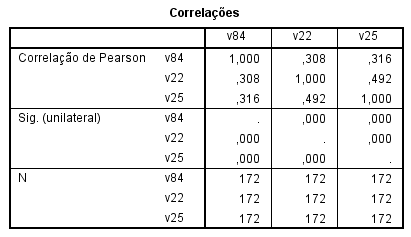
\includegraphics[height=5cm]{images/rl_multicolinearidade}
			\end{figure}

	\subsection{Análise de Outlier}
	
		``A identificação de outliers no modelo de regressão linear é feita essencialmente através dos \textbf{resíduos standardizados} (\emph{Standardized Residual - ZRE}), \textbf{studantizados} (\emph{Studentized Residual - SRE}) e \textbf{studantizados deletedos} (\emph{Studentized Deleted Residual - SDR}), pela verificação de pelo menos uma das condições:

		\begin{enumerate}[label=(\alph*)]
		
			\item Resíduos standardizados terem valores absolutos superiores a 3;			
			\item Resíduos studantizados terem valores absolutos superiores a 2;
			\item resíduos studantizados deleted terem valores absolutos superiores a 2". \cite{torres}
			
		\end{enumerate}

		Para isso gere \textbf{gráficos de linha simples} com as variáveis acima mencionadas com as seguintes configurações:
			
		Escala do gráfico: Mínimo: -4; Máximo: 4; Incremento: 1;

		Linhas de referências no eixo Y: ZRE: 3 e -3; SRE e SDR: 2 e -2.
			
		\begin{figure}[H]
			\centering
			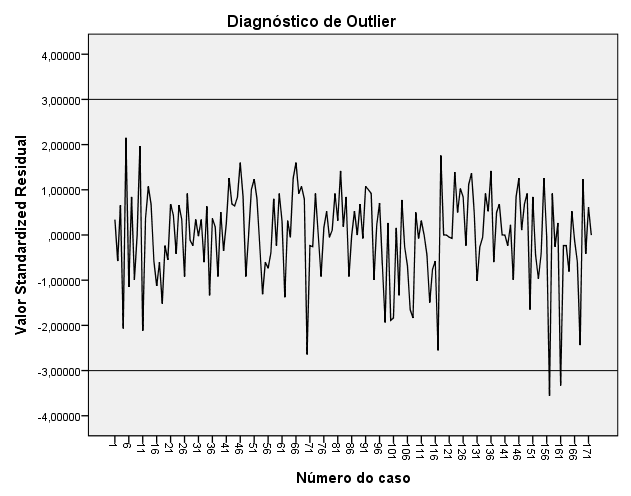
\includegraphics[height=6cm]{images/rl_analise-outlier_ZRE}
			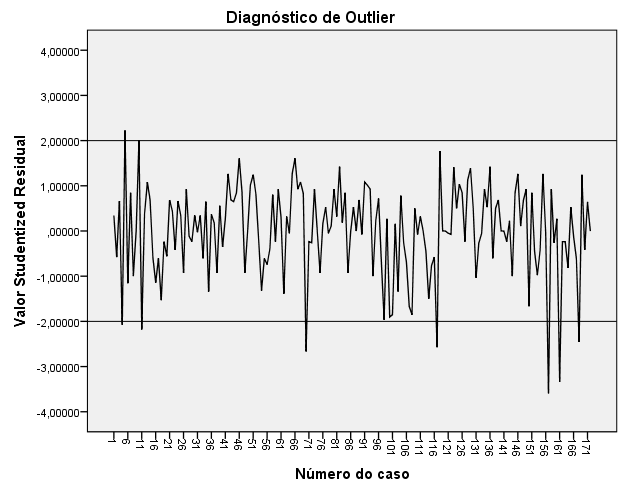
\includegraphics[height=6cm]{images/rl_analise-outlier_SRE}
			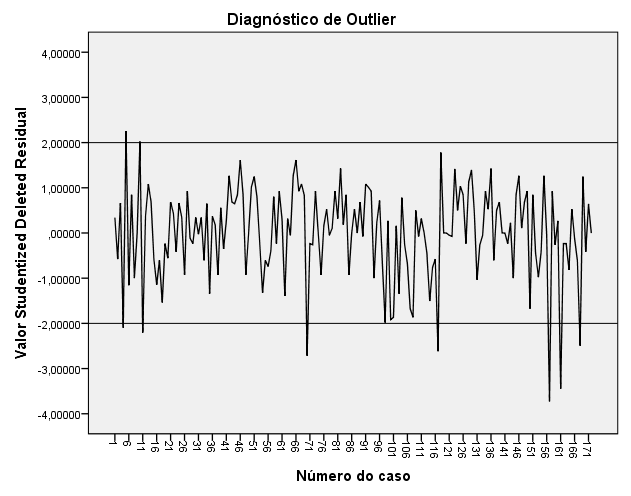
\includegraphics[height=6cm]{images/rl_analise-outlier_SRD}

		\end{figure}
			
		\textbf{Como remover os Outliers}

		\bigskip
				
		Comece tirando os outllies que aparecerem mais de um vez OU aqueles que a distância da linha de referência for maior - retire do $ n $ de número maior para o menor. Isso é importante pois o SPSS altera o número das linhas conforme você deleta o outlier.

		Rode o modelo de novo e veja se melhorou. Se não, retire mais outliers e repita o processo.

		Se você tirar muitos outliers você pode acabar com seu banco de dados. Caso isso aconteça um outra solução deve ser aplicada. Pode ser que colocando mais variáveis esse outliers melhorem (PODE SER).